%!TEX root = ../thesis.tex
%Adding the above line, with the name of your base .tex file (in this case "thesis.tex") will allow you to compile the whole thesis even when working inside one of the chapter tex files

\chapter{Multi-wavelength Study of Betelgeuse's Outer Atmosphere} \label{chap:5}

In this chapter we present the results from our multi-wavelength high resolution study of Betelgeuse's extended atmosphere. The majority of this chapter is based on the findings of \cite{ogorman_2012} and detail the results of our sub-arcsecond resolution study into the distribution and kinematics of CO\footnote{Throughout this chapter the usage of the term CO refers to the molecular isotope $^{12}$C$^{16}$O.} around Betelgeuse using the CO($J=2-1$) rotational line as the main probe. The variation of the emission line profile with different CARMA array configurations provides us with a unique insight into the distribution and kinematics of the two previously known flows, S1 and S2, around Betelgeuse. We successfully image the star on spatial scales as small as $0\arcsec .9$ ($\sim 20\,R_{\star}$) over a $32\arcsec$ ($\sim 750\,R_{\star}$) field of view and we discuss these radio maps in detail. We compare these results to higher CO rotational lines obtained with other instruments. We also present the recent findings of \cite{richards_2013} who image two distinct chromospheric features at centimeter wavelengths. These surprising findings motivated us to re-analyze old VLA-Pie Town data to search for these features at shorter wavelengths with comparable resolution, the results of which are presented at the end of this chapter. 

\section{CO molecules in the CSE of Betelgeuse}
\label{sec:5.1}
The CSE of Betelgeuse ($\alpha$ Ori) is a proving ground for ideas and theories of mass loss from oxygen-rich M-type supergiants. Currently it is losing mass at a respectable rate $\sim 2\times 10^{-6} \ M_{\odot}$ yr${}^{-1}$ \citep{harper_2001}, as it has been over the past $\sim$ 1000 years. Most of the optically thin silicate dust lies beyond $\sim 46$ stellar radii \citep{danchi_1994} and dust is, therefore, unlikely to be responsible for the bulk mass loss. This raises the important point that if the mass loss from Betelgeuse is not a result of dust then perhaps the same mechanisms that are responsible might also be active in the more dusty later M-type supergiants. Radiation pressure on atoms and molecules is another potential contributing candidate as a mass loss mechanism and so spatial and dynamical studies of molecules are a fruitful line of investigation, especially in relation to eventual formation of dust. Such studies also allow us to calculate the time scales on which certain mass loss episodes have occurred, and these can then be compared to the time scales of potential mass-loss initiators such as convection or magnetic dynamo cycles.

Despite the initial reports of an enhancement of C abundance in its atmosphere \citep{spinrad_1966}, Betelgeuse is now known to be an oxygen-rich star. The comprehensive study of CO and OH ro-vibrational bands by \cite{lambert_1984} found log\,$\epsilon$(C) $ = 8.4$ and log\,$\epsilon$(O)$ = 8.8$. For any species X
\begin{equation}
\rm{log}\,\epsilon(X)=\rm{log}\,(X/H)+12,
\end{equation}
which can be used to show O/C$ = 2.5$. \cite{lambert_1984} also found log\,$\epsilon$(N)$ = 8.6$ which indicates a contamination of the atmosphere with C-N processed material. This is in agreement with the theoretical work of \cite{lamb_1976} who predict the dredging up of processed material by the deep convective envelope which a supergiant like Betelgeuse is expected to possess. Betelgeuse is unlikely to have undergone a second dredge-up of material that would cause small changes in the CNO abundances due to its mass being greater than the upper mass limit for a second dredge-up to occur.  This second dredge-up is predicted to occur after He core exhaustion for stars below $8-10 \,M_{\odot}$ \citep{kaler_1978}. The observed $^{12}$C/$^{13}$C ratio, which is an indication of the history of nuclear processing and mixing in the interior of stars \citep{pavlenko_2003,eggleton_2007} has consistently found to be between 6 and 7 \citep{lambert_1974,hinkle_1976,bernat_1979,harris_1984}, well below the predicted value of 20 \citep{charbonnel_1995,pavlenko_2003}, which is the case for most red giant stars \citep[e.g.,][]{boothroyd_1999}.

\begin{figure}[!ht]
\centering 
          \includegraphics[trim=120pt 230pt 120pt 200pt,clip,scale=0.6]{/home/eamon/thesis/thesis_template/5/bernat_new.ps}
\caption[Bernat (1979) CO line profile showing two sharp line cores.]{CO ro-vibrational fundamental line showing two sharp blueshifted absorption features originating from the expanding envelope \citep{bernat_1979}. These two features became known as the S1 and S2 components of Betelgeuse's outflow having outflow velocities of $\sim 9$ and $\sim 16$\, km\,s$^{-1}$, respectively. The units of the x-axis are cm$^{-1}$.}
\label{fig:5.1}
\end{figure}

The study of CO molecules in the CSE of Betelgeuse began with the detection of 4.6\,$\mu$m ro-vibrational absorption lines of $\rm{{}^{12}C^{16}O}$ and $\rm{{}^{13}C^{16}O}$ by \cite{bernat_1979} who identified two absorption features shown in Figure \ref{fig:5.1}, implying two distinct components within the overall outflow. One component, known as S1, has a Doppler shift of $9\>{\rm km\>s}^{-1}$ towards us with T$_{\rm{exc}}\,\simeq\,200\,\rm{K}$, $v_{\rm{turb}}\,\simeq\,4$\,km\,s${}^{-1}$, and N$_{\rm{CO}}=4.7\times 10^{17}\>{\rm cm}^{-2}$. The second faster component, known as S2, has a Doppler shift of $16\>{\rm km\>s}^{-1}$ towards us with T$_{\rm{exc}} \simeq$ 70 $\rm{K}$, $v_{\rm{turb}}\simeq 1$\,km\,s${}^{-1}$, and N$_{\rm{CO}}=1.2\times 10^{16}\>{\rm cm}^{-2}$. \cite{bernat_1979} noted that a simple assumption of the dust and gas being in thermal equilibrium would infer that the S1 and S2 components have a spatial extent of 4 and $55\arcsec$ respectively, using the dust model of \cite{tsuji_1979}. The S1 feature with its higher column density was well known from atomic absorption line studies \citep[e.g.][]{weymann_1962} and both features had been detected in high spectral resolution atomic Na and K absorption profiles \citep{goldberg_1975}.

\begin{figure}[!ht]
\centering 
\mbox{
          \includegraphics[trim=40pt 240pt 50pt 230pt,clip,width=7.0cm,height=6.0cm]{/home/eamon/thesis/thesis_template/5/huggins_1987.ps}
          \includegraphics[trim=30pt 250pt 20pt 200pt,clip,width=7.5cm,height=6.5cm]{/home/eamon/thesis/thesis_template/5/huggins_1994.ps}
          }
\caption[Previous CO$J= 2-1$ rotational emission line profiles]{Previous single dish CO($J= 2-1$) rotational emission line profiles of Betelgeuse. \textit{Left:} \cite{huggins_1987} line profile using a HPBW of 32$\arcsec$. They found some evidence for an S2 radius of about $16\arcsec$. \textit{Right:} The line of \cite{huggins_1994} looks very similar even using a smaller HPBW in conflict with the findings of \cite{huggins_1987}. Velocities are plotted in the local standard of rest (LSR) frame.}
\label{fig:5.2}
\end{figure}

CO was first detected at radio wavelengths by \cite{knapp_1980} who presented a low S/N ratio spectrum of the $J= 2-1$ rotational emission line at 230\,GHz. They used a single dish antenna with a HPBW of $\sim 30\arcsec$ and detected one component expanding at 15\,km\,s$^{-1}$. They assumed this component to be the S2 component detected by  \cite{bernat_1979} and by assuming that they had resolved a flat top profile, predicted that its spatial extent didn't exceed $10\arcsec$. The weaker CO($J=1-0$) line was tentatively detected by \cite{knapp_1985} with a 7\,m dish which had a HPBW of 100$\arcsec$. \cite{huggins_1987} presented a higher signal-to-noise CO($J=2-1$) profile that was obtained with a HPBW of 32$\arcsec$ and is shown in Figure \ref{fig:5.2}. By comparing the  $(2-1)/(1-0)$ line intensities they found some evidence for an S2 radius of $\sim 16\arcsec$. However,  a 30\,m IRAM $J= 2-1$ line profile was later presented by \cite{huggins_1994} and as can be seen in Figure \ref{fig:5.2} looked remarkably similar, even though it was observed with a smaller 12$\arcsec$ HPBW. The profile did not show the horned wing signature expected if it had been resolved as discussed in Chapter 1, apparently in conflict with the previous S2 radius estimate. These single dish line profiles also showed no signature of the slower S1 shell and so questions remained about the spatial extent of these two distinct outflow components in the CSE of Betelgeuse. A sensitive high spatial resolution study of it's atmosphere was needed to untangle this puzzling evidence.

\section{Adopted Radial Velocity}\label{sec:5.2}

Before we discuss the CO($J=2-1$) spectra obtained from our multi-configuration CARMA observations which are summarized in Chapter 3, we begin by explaining which radial velocity value $v_{\rm{rad}}$, for Betelgeuse was adopted. An accurate value of $v_{\rm{rad}}$ is necessary when plotting the spectra of any star with respect to its center of mass rest frame, as we do for all spectra in this chapter. Plotting spectra in this frame of reference is intuitive as it allows the reader to immediately see the gas expansion velocity relative to the photosphere. A positive $v_{\rm{rad}}$ denotes recession (i.e., redshifted lines) while a negative $v_{\rm{rad}}$ denotes advancement (i.e., blueshifted lines).

Betelgeuse is a  semi-regular variable and its radial velocity exhibits variability on time scales ranging from short 1.5 year periods as suggested by \cite{stebbins_1931} to longer 5.8 year periods \citep{spencer_jones_1928,smith_1989}. 
\cite{stothers_1971} interpreted the long period as being the convective turnover time of giant convection cells on the stellar surface while \cite{dupree_1990} attribute the shorter period with pulsation. Betelgeuse's radial velocity amplitudes are also known to vary by at least $\pm 3\>{\rm km\>s}^{-1}$ \citep{smith_1989} making it difficult to determine a precise value for the stellar center of mass radial velocity. In Figure \ref{fig:5.3} we plot the radial velocity data and the corresponding model derived in the classical paper by \cite{sanford_1933} which is based on observations spanning 1923 to 1931. We have also extrapolated the model back to show that it matches the earlier data of \cite{bottlinger_1911} and \cite{spencer_jones_1928} quite well, as shown in Figure \ref{fig:5.3}. \cite{goldberg_1984} has also shown that the model of \cite{sanford_1933} can be extrapolated forward to give a reasonable fit to his measurements. In this study we adopt a heliocentric radial velocity of $+20.7\>{\rm km\>s}^{-1}$;  a value used by \cite{weymann_1962} and \citet{harper_2008} and is based on the mean values of \cite{spencer_jones_1928} and \cite{sanford_1933} radial velocity models. 

\begin{figure}[!ht]
\centering 
\mbox{
          \includegraphics[trim=0pt 0pt 0pt 50pt,clip,angle=90,height=7.0cm,width=7.3cm]{/home/eamon/thesis/thesis_template/5/vrad1.ps}
          \includegraphics[trim=0pt 0pt 0pt 50pt,clip,angle=90,height=7.0cm,width=7.3cm]{/home/eamon/thesis/thesis_template/5/vrad2.ps}
          }
\caption[Radial velocity data and model for $\alpha$ Ori.]{The radial velocity model of \cite{sanford_1933} along with measurements from \cite{bottlinger_1911}, \cite{spencer_jones_1928}, and \cite{sanford_1933} spanning from $1897 - 1931$. In this study we use $+20.7\>{\rm km\>s}^{-1}$ which is the mean value from the models of \cite{spencer_jones_1928} and \cite{sanford_1933}. The radial velocity amplitude variations of $\sim \pm 3\>{\rm km\>s}^{-1}$ is clearly evident in these data.}
\label{fig:5.3}
\end{figure}

\section{CARMA CO($J=2-1$) Spectra}
\label{sec:5.3}

The spectrum for each individual configuration image cube (which are composed of all the appropriate configuration tracks listed in Table \ref{tab:3.3}) along with the multi-configuration image cube (which is composed of the entire data set  spanning $\sim 2.5$\,yr) can be used to obtain information on the kinematics of the S1 and S2 flows. In particular, it is of interest to see how the CO($J=2-1$) line profile changes when observed  with different array configurations as each of these will be sensitive to emission on different spatial scales. . The spectra corresponding  to the C, D, and E configuration image cubes are plotted in Figure \ref{fig:5.4} for both the high ($0.65\>{\rm km\>s}^{-1}\> \rm{bin}^{-1}$) and low ($1.3\>{\rm km\>s}^{-1}\> \rm{bin}^{-1}$) spectral resolution data and were obtained by integrating all emission within a circular area of radius 5$\arcsec$ centered on the source. The high and low spectral resolution modes allow two independent sets of spectra to be measured for each observation and thus provide a good check on the data quality. The high resolution  spectra (channel width = $0.65\>{\rm km\>s}^{-1}$) give the best measure of the S1 and S2 flow kinematics and therefore all outflow velocities are derived from these spectra.
%Prior to this study, the line had only ever been observed with single dish antennas and so the resolution was set by the HPBW of the antenna used, the maximum being the $12\arcsec$ HPBW beam of \cite{huggins_1994}

\begin{figure}[!ht]
\centering 
\includegraphics[trim=80pt 60pt 40pt 80pt, clip, width=9.0cm, height=12.0cm]{/home/eamon/thesis/thesis_template/5/f1.eps}
\caption{Spectra integrated over a radius of 5$\arcsec$ for each array configuration image cube. The blueshifted emission component between $-16.0\>{\rm km\>s}^{-1}$ and $-10.0\>{\rm km\>s}^{-1}$ is almost resolved out in the C configuration image cube spectrum. The red and blue lines correspond to the high and low spectral resolution data respectively.}
\label{fig:5.4}
\end{figure}

The E configuration image cube spectrum has a total line width of $29.2\>{\rm km\>s}^{-1}$ and the low spectral resolution profile contains a steep blue wing emission feature between $-16.0\>{\rm km\>s}^{-1}$ and $-11\>{\rm km\>s}^{-1}$ and a more flat-topped feature between $-10.3\>{\rm km\>s}^{-1}$ and $-13.2\>{\rm km\>s}^{-1}$. This steep emission wing shows that the turbulence in the flow is less than or equal to the velocity bin size. The blue wing in the high resolution profile matches the lower resolution profile well but the remainder of the profile looks more complex than the flat-topped feature seen in the lower resolution profile. The line profile shape has been well documented by previous single dish observations (e.g., Figure \ref{fig:5.2}) and, out of our three individual configuration spectra, we expect the most compact E configuration spectra to resemble these single dish measurements the closest due to its better sampling of the inner $u-v$ plane and consequent sensitivity to extended structures. This indeed turns out to be the case when we compare our three individual configuration spectra to those previous single dish profiles. The blue wing emission feature appears again in the D configuration spectrum at the same velocities as those in the E configuration spectrum but the remainder of the profile appears quite different. Between $-10.3\>{\rm km\>s}^{-1}$ and $+13.2\>{\rm km\>s}^{-1}$ the D configuration spectrum is dominated by a blue wing at $\sim$ $-10.0\>{\rm km\>s}^{-1}$, a red wing at $\sim$ $+13.0\>{\rm km\>s}^{-1}$ and an emission feature at $\sim$ $0\>{\rm km\>s}^{-1}$. The large drop in emission at certain velocities in the D configuration spectrum is probably a result of the lower sensitivity to large scale structure in comparison to the E configuration as described in Table \ref{tab:3.2}.

The line profile has a lower flux ($\sim 50\,\%$) in the high spatial resolution C configuration spectrum due to its lack of sensitivity to extended structure. Notably, the blueshifted emission feature located between $-16.0\>{\rm km\>s}^{-1}$ and $-11.0\>{\rm km\>s}^{-1}$ in the E and D configuration spectra is almost completely spatially filtered by the extended C configuration. This component of the line has previously been associated with the outer S2 flow \citep{huggins_1987} and as the majority of it has been spatially filtered by our C configuration we expect even less contribution from the S2 flow at lower absolute velocities still. For the redshifted line emission we again expect the majority of the S2 contribution to be spatially filtered, so we conclude that most, if not all of the emission in the C configuration spectrum emanates from the inner S1 flow. The spectrum is double peaked with the blue and redshifted wings extending to $-9.0\>{\rm km\>s}^{-1}$ and $+10.6\>{\rm km\>s}^{-1}$ respectively, and we define these as the outflow velocities of S1. As discussed in Chapter \ref{chap:3} the C configuration has a resolving out scale of $\sim$ 6$\arcsec$ at 1.3 mm and so is not sensitive to angular scales larger than this. If the emission between $-9.0\>{\rm km\>s}^{-1}$ and $+10.6\>{\rm km\>s}^{-1}$ in the C configuration spectrum appeared as a flat topped profile then we could conclude that the S1 flow lies within a radius of 3$\arcsec$ from the star. Clearly however, the profile has a more \textit{horned} shaped appearance and so the lower absolute velocity components of this profile have been spatially filtered. We can therefore conclude that the radial extent of the S1 from the star is greater than 3$\arcsec$. If we assume that the S1 flow would produce a 19.6 $\pm$ $0.7\>{\rm km\>s}^{-1}$ wide top-hat line profile of 2 mJy were it not for the resolving out effects of the interferometer, its integrated line flux is then
\begin{equation}
F_{\rm{tot\,S1}}=F_{\nu}\times \left(\frac{\Delta v}{\lambda}\right)= 3.1 \times 10{}^{-19}\,\rm{W\,m}{}^{-2}.
\label{eq:5.1}
\end{equation}

To obtain the most robust value for the S2 outflow velocities we examine the high spectral resolution multi-configuration image cube spectrum which is composed of all tracks from all three configurations. It is worth stressing that by analyzing the multi-configuration image cube we make the assumption that the physical properties of all three components (i.e. $\alpha$ Ori, S1 and S2) have not changed over the total observation period (i.e. $\sim$ 2.5 yr). The profile is found to have a total linewidth of 28.6 $\pm$ $0.7\>{\rm km\>s}^{-1}$, which is in good agreement with previous single dish observations of the line where values of 30.6 $\pm$ $2.5\>{\rm km\>s}^{-1}$ and $28.6\>{\rm km\>s}^{-1}$ were reported by \cite{knapp_1980} and \cite{huggins_1987} respectively. The centroid velocity of the spectrum is  $-1.1 \pm 0.7$ km s$^{-1}$ ($\rm{v_{\rm{lsr}}}$ = 3.7 $\pm$ $0.7\>{\rm km\>s}^{-1}$) which again is in good agreement with \cite{knapp_1980} and \cite{huggins_1987} values of $\rm{v_{lsr}}$ = 3.0 $\pm$ $2.5\>{\rm km\>s}^{-1}$ and $\rm{v_{lsr}}$ = 3.7 $\pm$ $0.4\>{\rm km\>s}^{-1}$, respectively. We use Equation \ref{eq:5.1} to find the integrated total line flux to be 1.5 $\times 10^{-18}$\,W\,m$^{-2}$, of which at least 20\% emanates from the S1 flow.

\begin{figure}[!ht]
\centering 
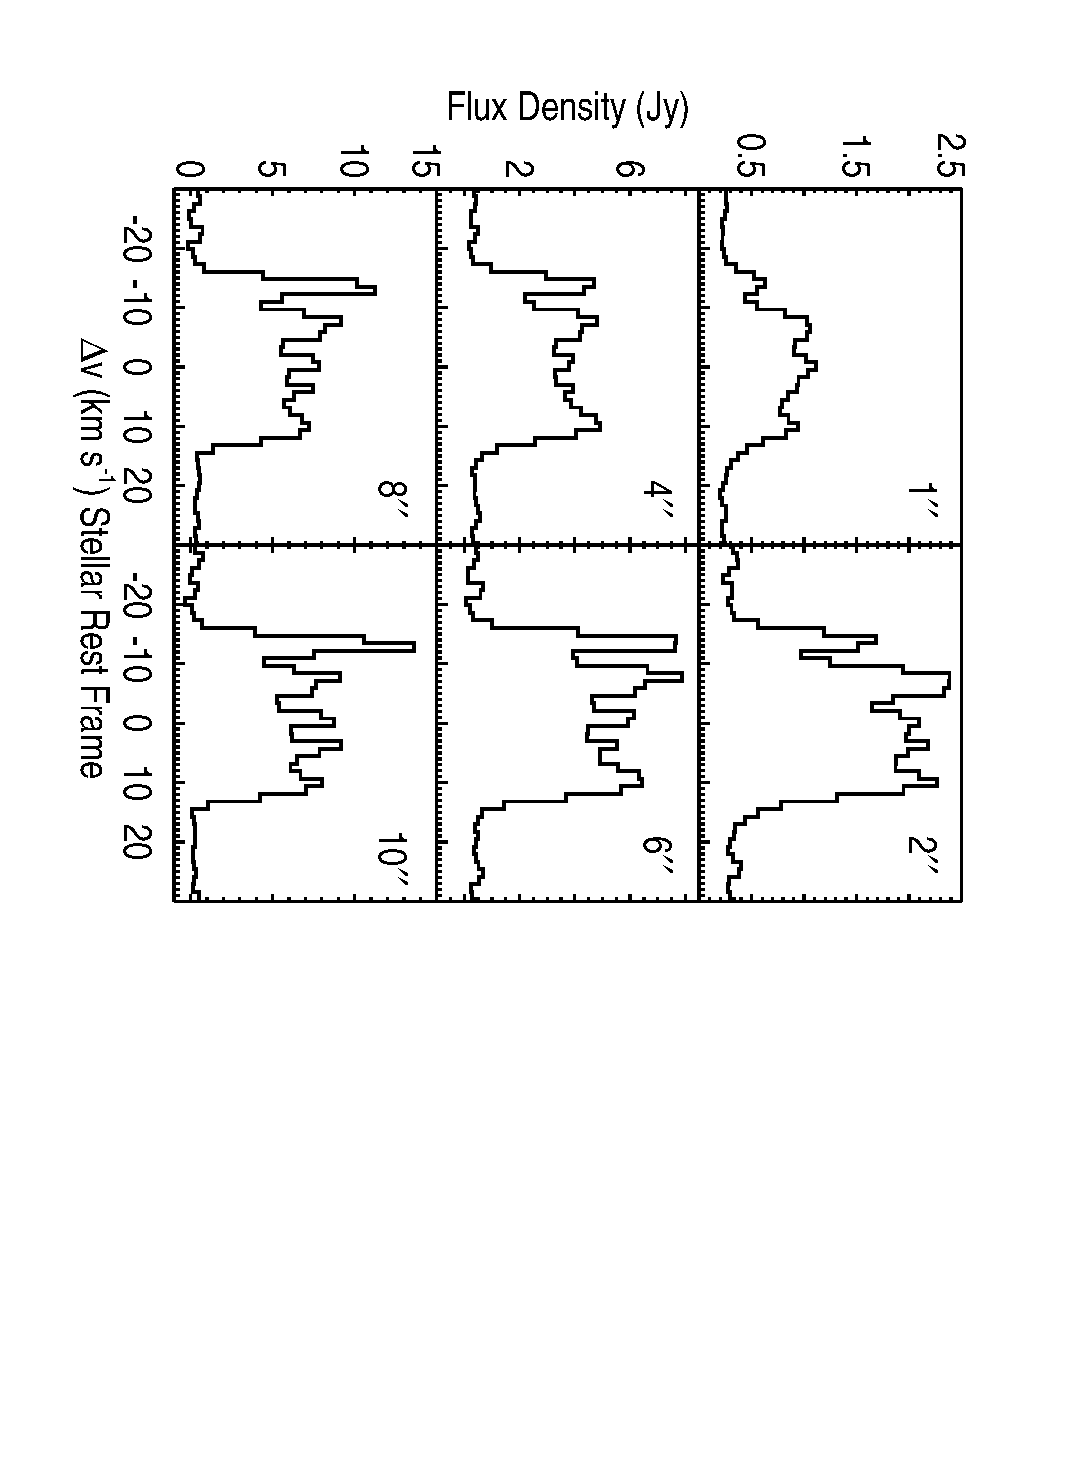
\includegraphics[trim=20pt 180pt 40pt 0pt, clip, angle=90, width=14.0cm, height=12.0cm]{/home/eamon/thesis/thesis_template/5/f2.eps}
\caption{Spectral profiles of the low spectral resolution multi-configuration image cube for circular extraction areas of radius 1$\arcsec$, 2$\arcsec$, 4$\arcsec$, 6$\arcsec$, 8$\arcsec$, and 10$\arcsec$. The signal-to-noise of the line profile reduces at larger extraction areas as more noise is included from the outer regions of the channel maps.}
\label{fig:5.5}
\end{figure}

The outflow velocities of S2 are $-15.4\>{\rm km\>s}^{-1}$ and $+13.2\>{\rm km\>s}^{-1}$ which, like the S1 flow, are slightly asymmetric but in the opposite sense. Note that the S1 and S2 outflow velocities are dependent on the adopted radial velocity of Betelgeuse. If for instance, we instead adopt a radial velocity of 21.9 km s${}^{-1}$ \citep{famaey_2005} then the the S2 outflow velocities become even more asymmetric (-16.6 and $+12.0\>{\rm km\>s}^{-1}$) while the S1 outflow becomes less so (-10.2 and $+9.4\>{\rm km\>s}^{-1}$). Both S1 and S2 therefore cannot have spherically symmetric outflow velocities regardless of the adopted stellar radial velocity. Adopting a mass of 18\,$M_{\odot}$ \citep{meynet_2003} and a radius of 950\,$R_{\odot}$ \citep{harper_2008} then the escape velocity for Betelgeuse is $85\>{\rm km\>s}^{-1}$ which is much greater than the S1 and S2 outflow velocities. This indicates that the majority of the stellar mass loss mechanism's energy goes into lifting the CO molecules out of the gravitational potential and not into their outflow velocities. These outflow velocities are greater than the adiabatic hydrogen sound speed (i.e., $11.7\sqrt{10^{-4}T_{e}}$), which, if we assume that the gas temperature is the same as the excitation temperature, are $1.7\>{\rm km\>s}^{-1}$ and $1\>{\rm km\>s}^{-1}$ for S1 and S2 respectively. 

The spectra in Figure \ref{fig:5.5} are taken from the low resolution multi-configuration image cube using circular extraction areas ranging in radius from 1$\arcsec$ to 10$\arcsec$ and demonstrates how the line profile changes over these different extraction areas. The most striking change in the line profile is the change in appearance of the extreme blue wing. At small extraction radii where we sample the most compact emission, the feature is weak in comparison to the rest of the line but becomes more dominant as we begin to sample more of the extended emission. This indicates that even the high absolute velocity components of the S2 flow have extended emission and this is why they are almost completely spatially filtered by CARMA's C configuration. The large reduction of flux at $-11\>{\rm km\>s}^{-1}$ suggests that there is more material moving towards the observer than at other lower absolute velocities indicating a non-isotropic (or non-spherical) S2 flow. This suggests a more sheet like (flatter) structure rather than a spherical cap.

\section{Individual Configuration Image Cubes}\label{sec:5.4}

\begin{figure}[htp]
\mbox{
          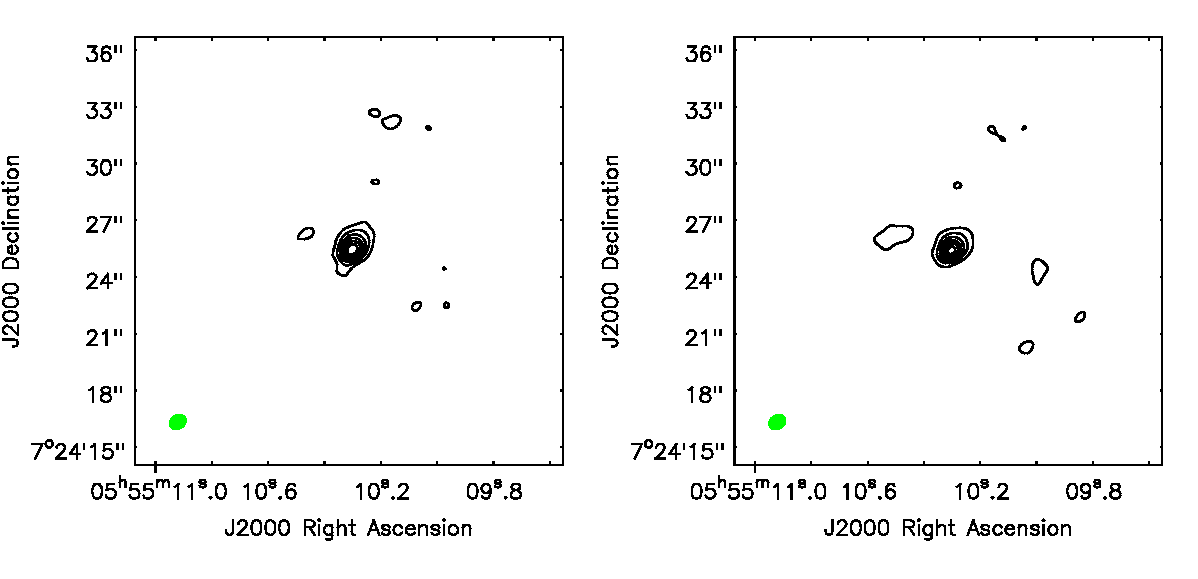
\includegraphics[trim=0pt 0pt 10pt 10pt,clip,height=6.2cm,width=14.0cm]{/home/eamon/thesis/thesis_template/5/c.ps}
          }
\mbox{
          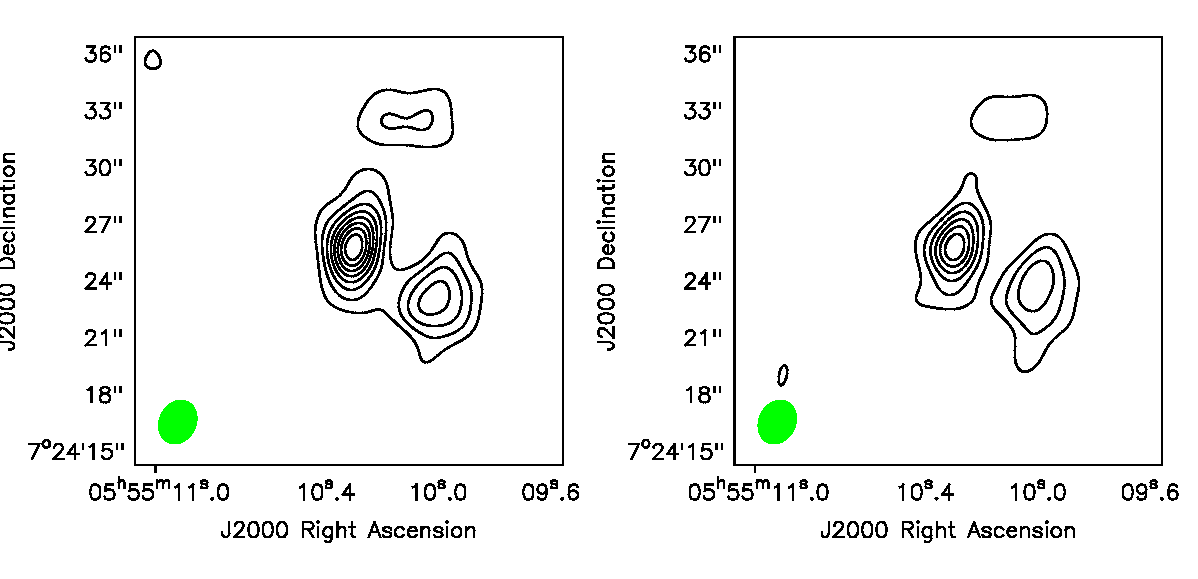
\includegraphics[trim=0pt 0pt 10pt 10pt,clip,height=6.2cm,width=14.0cm]{/home/eamon/thesis/thesis_template/5/d.ps}
          }
\mbox{
          \includegraphics[trim=0pt 0pt 10pt 10pt,clip,height=6.2cm,width=14.0cm]{/home/eamon/thesis/thesis_template/5/e.ps}
          }          
\caption[Discrete sources in individual configuration image cubes]{Two channel maps from each of the three individual configuration image cubes. A spatially unresolved source is present in five continuous channel maps between $\sim$ $-4.0\>{\rm km\>s}^{-1}$ and $+2.4\>{\rm km\>s}^{-1}$ and is located $\sim$ 5$\arcsec$ S-W of $\alpha$ Ori. Contour levels begin at $4\sigma$ where $1\sigma$ is the rms channel noise. The restoring beam is shown in green in the lower left corner of each map.}
\label{fig:5.6}
\end{figure}

We created three image cubes for each configuration by concatenating all good tracks together per configuration. The gradual formation of a ring type structure as one goes from high absolute velocities to lower absolute velocities indicative of a shell was not seen in any of these three image cubes. However, an additional spatially unresolved source was clearly detected in a number of the D configuration image cube maps (both high and low spectral resolution). The component is present in five continuous channel maps between $\sim$ $-4.0\>{\rm km\>s}^{-1}$ and $+2.4\>{\rm km\>s}^{-1}$ and is located $\sim$ 5$\arcsec$ S-W of $\alpha$ Ori. Its peak emission lies at $\sim$ $0\>{\rm km\>s}^{-1}$ and has a flux density of 1.8\,mJy which is approximately 60$\%$ of the total source flux density at this velocity. The middle row in Figure \ref{fig:5.6} are two of these D configuration channel maps which clearly show this discrete source. The contour levels are set at the $4\sigma$ level so the detection of the second source in the D configuration is significant. The corresponding channel maps in the E configuration image cube show extended emission out to ~8$\arcsec$ in the same S-W direction as can be seen in the lower panel of Figure \ref{fig:5.6}. There is only weak emission detected in the same position in the corresponding C configuration channel maps, probably due to the lower sensitivity resulting from the smaller HPBW (i.e., the flux is diluted). This discrete second source thus has the effect of adding extra emission to the corresponding multi-configuration image cube spectrum at the low absolute velocities where it is present. The presence of this addition source at these low absolute velocities is probably one of the reasons why \cite{huggins_1994} did not detect a horned shaped spectrum with his 12$\arcsec$ HPBW. We also note that that there is a weaker emission feature 7$\arcsec$ north north-west of $\alpha$ Ori in these maps also which too can be seen in Figure \ref{fig:5.6}. 

\section{Multi-configuration Image Cube Inspection}\label{sec:5.5}

%\begin{figure}[htp]
%\centering
%\mbox{
%          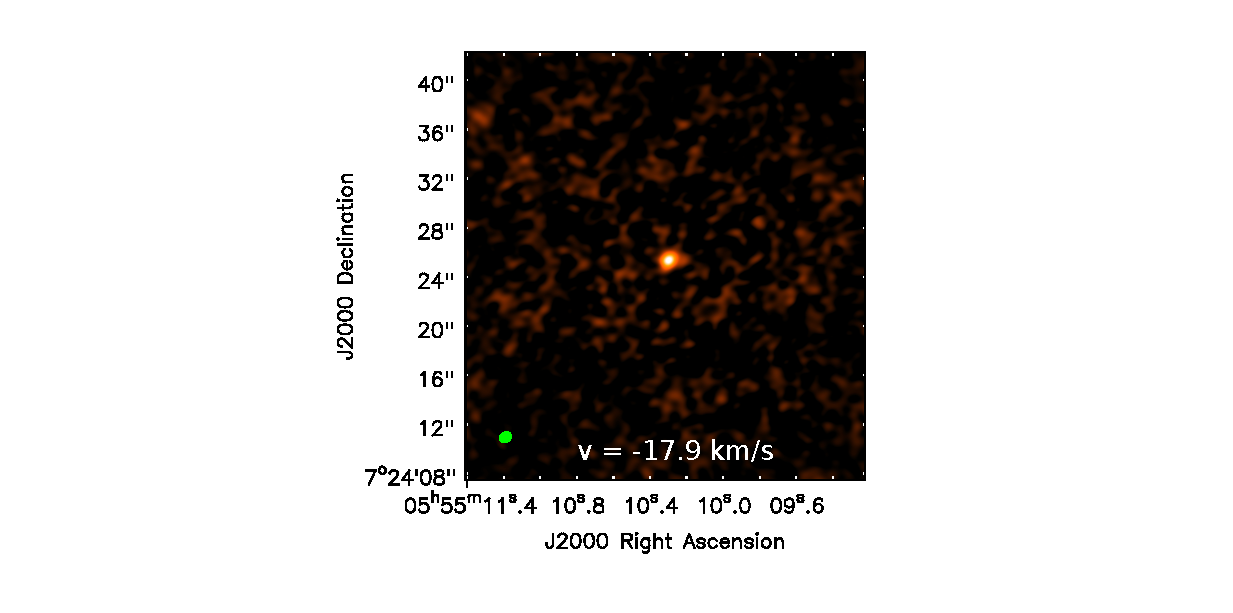
\includegraphics[trim=130pt 15pt 120pt 15pt,clip,scale=0.55]{/home/eamon/thesis/thesis_template/5/1.eps}
%          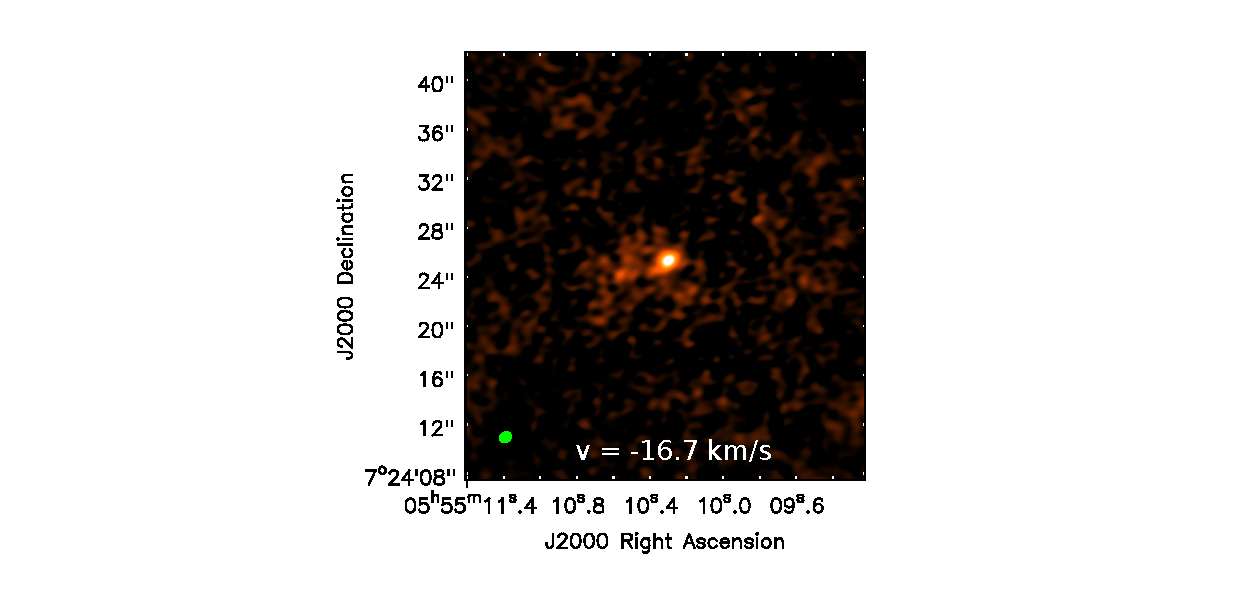
\includegraphics[trim=180pt 15pt 120pt 15pt,clip,scale=0.55]{/home/eamon/thesis/thesis_template/5/2.eps}
%         \includegraphics[trim=260pt 230pt 200pt 270pt,clip,scale=0.4]{/home/eamon/thesis/thesis_template/5/color_wedge.ps}
%          }
%\mbox{
%          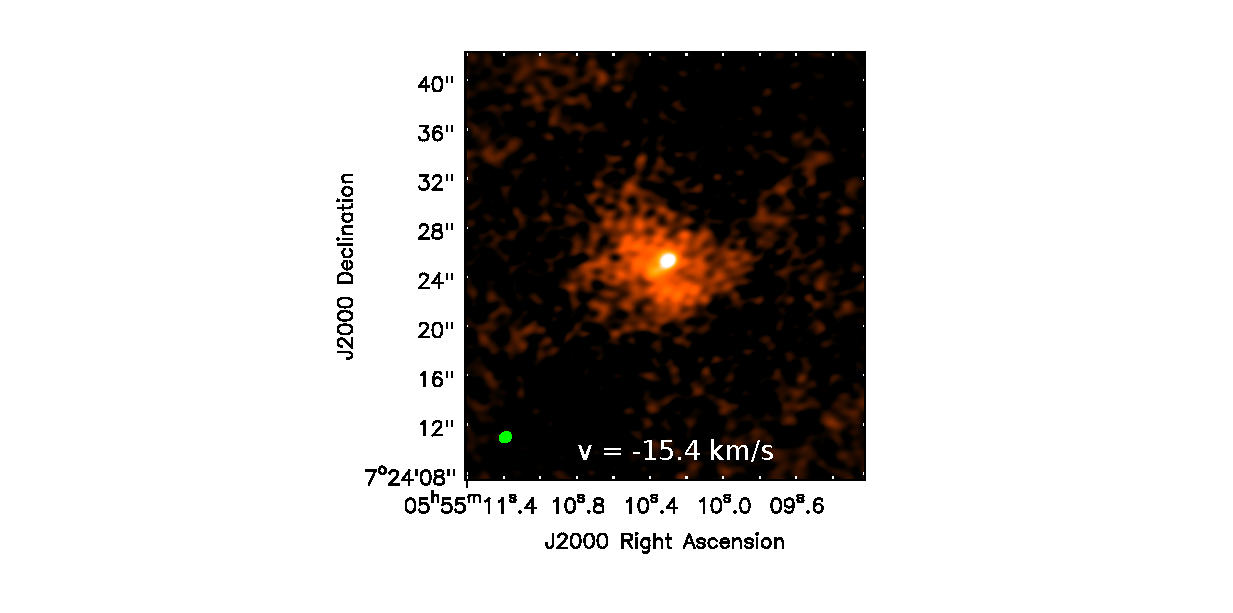
\includegraphics[trim=130pt 15pt 120pt 15pt,clip,scale=0.55]{/home/eamon/thesis/thesis_template/5/3.eps}
%          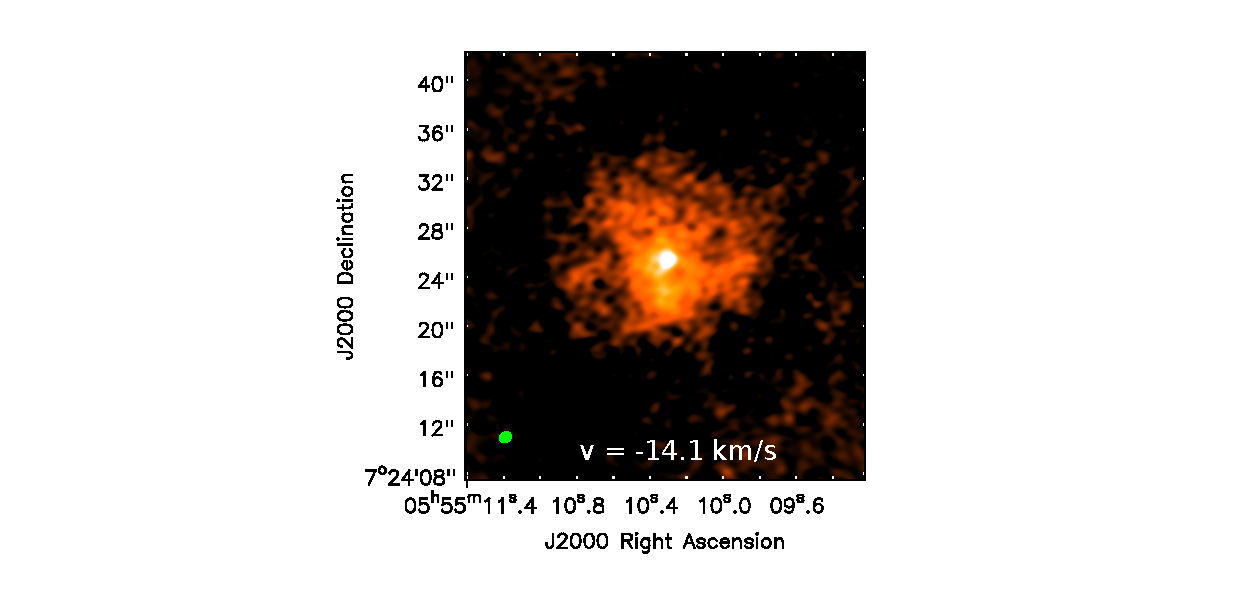
\includegraphics[trim=180pt 15pt 120pt 15pt,clip,scale=0.55]{/home/eamon/thesis/thesis_template/5/4.eps}
%          \includegraphics[trim=260pt 230pt 200pt 270pt,clip,scale=0.4]{/home/eamon/thesis/thesis_template/5/color_wedge.ps}
%          }
%\mbox{
%          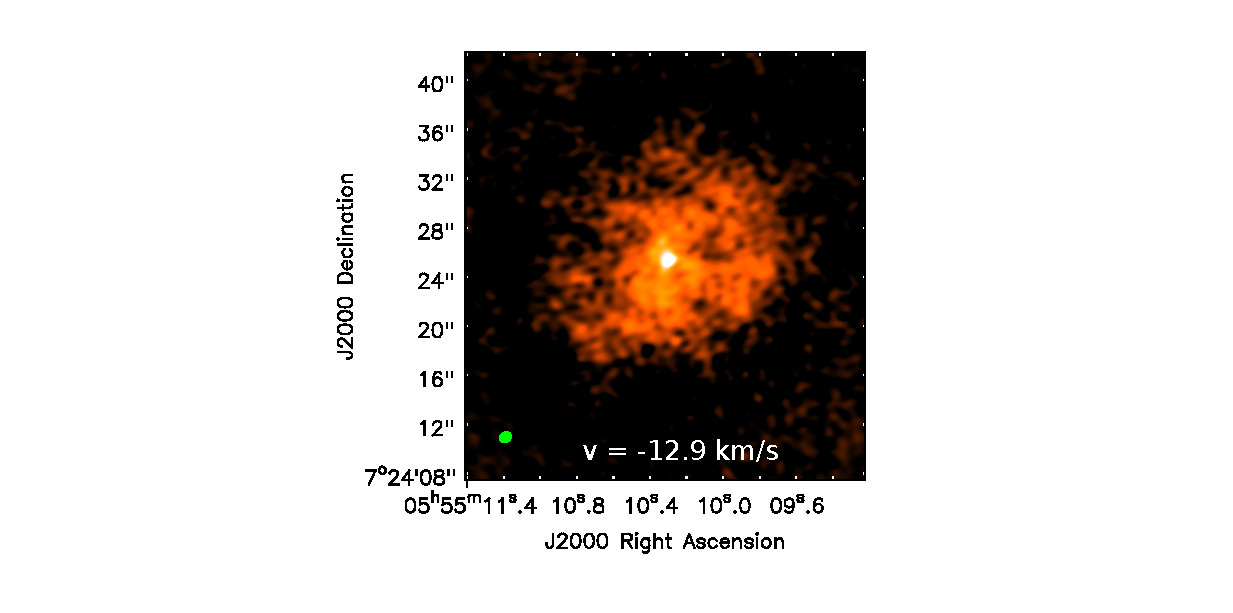
\includegraphics[trim=130pt 15pt 120pt 15pt,clip,scale=0.55]{/home/eamon/thesis/thesis_template/5/5.eps}
%          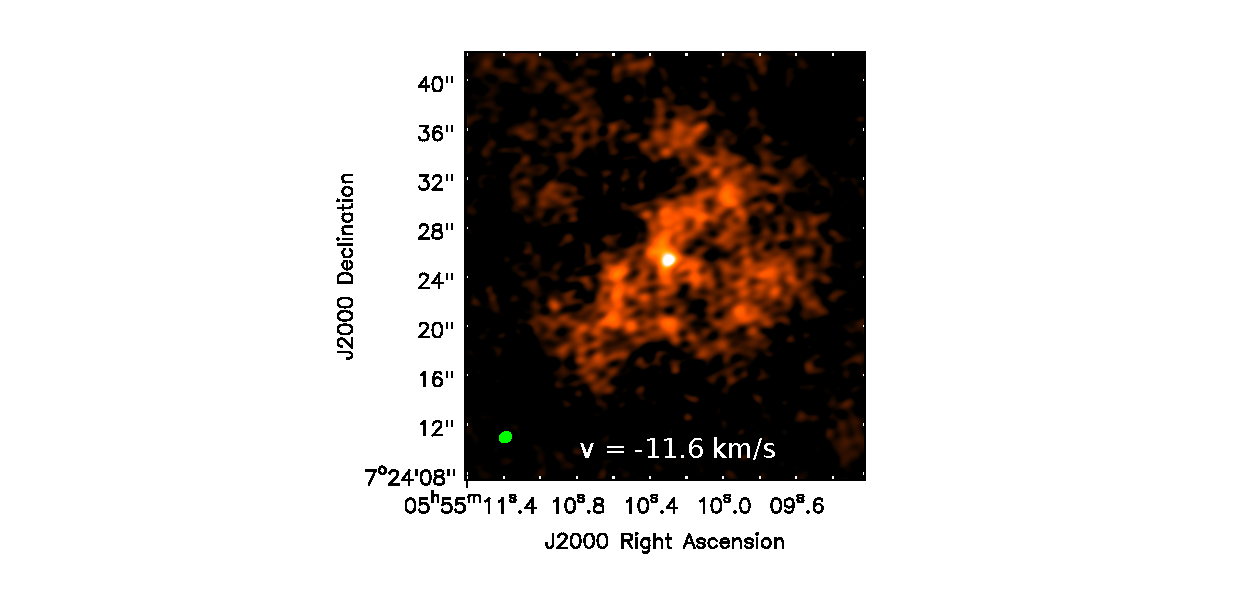
\includegraphics[trim=180pt 15pt 120pt 15pt,clip,scale=0.55]{/home/eamon/thesis/thesis_template/5/6.eps}
%          \includegraphics[trim=260pt 230pt 200pt 270pt,clip,scale=0.4]{/home/eamon/thesis/thesis_template/5/color_wedge.ps}
%          }
%\mbox{
%          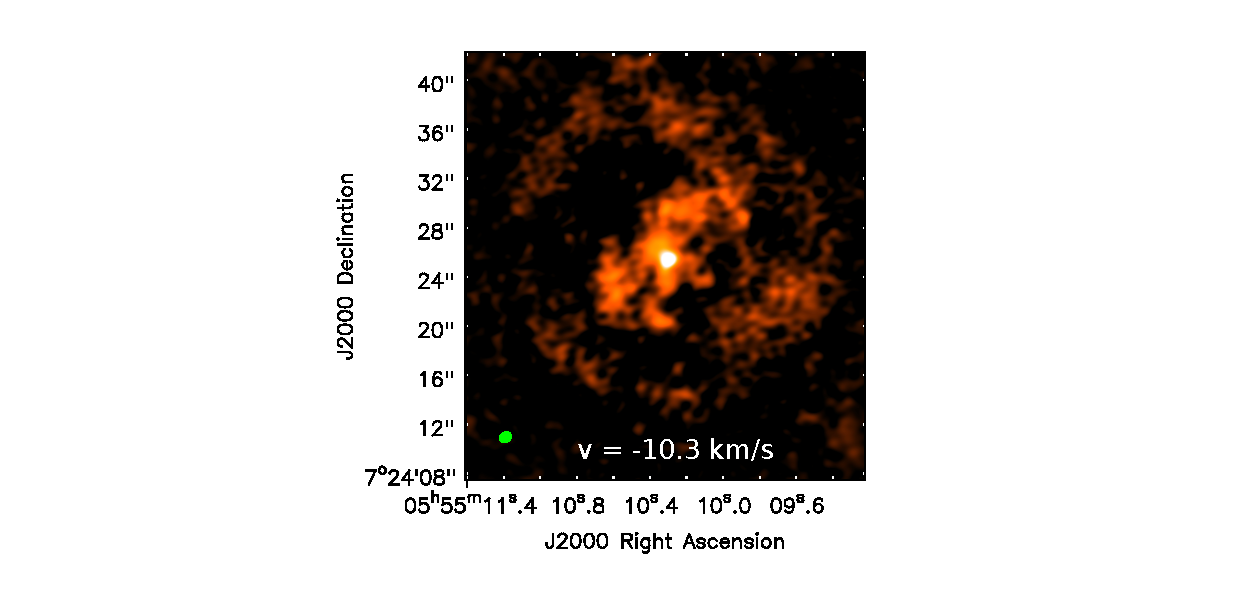
\includegraphics[trim=130pt 15pt 120pt 15pt,clip,scale=0.55]{/home/eamon/thesis/thesis_template/5/7.eps}
%          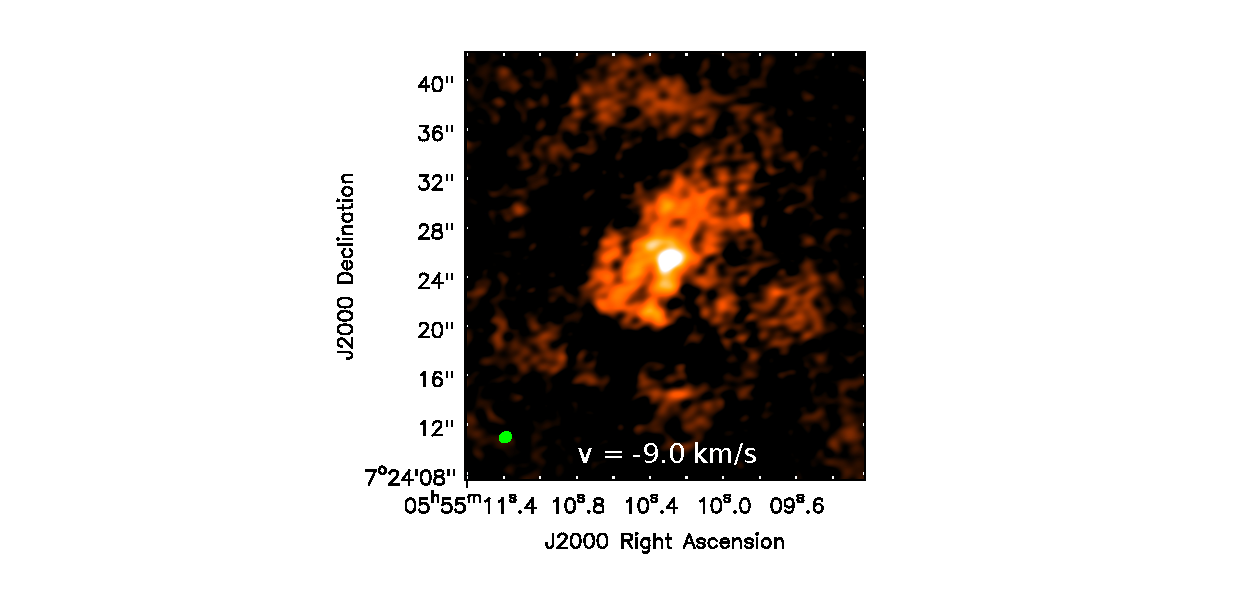
\includegraphics[trim=180pt 15pt 120pt 15pt,clip,scale=0.55]{/home/eamon/thesis/thesis_template/5/8.eps}
%          \includegraphics[trim=260pt 230pt 200pt 270pt,clip,scale=0.4]{/home/eamon/thesis/thesis_template/5/color_wedge.ps}
%          }                           
%\caption[Channel maps from the multi-configuration image cube]{8 channel maps from the multi-configuration image cube ($\Delta v$ = $1.3\>{\rm km\>s}^{-1}$). The peak emission has been cut at 0.2 Jy beam${{}^{-1}}$ to emphasize the fainter emission. The map at $-17.9$ km s$^{-1}$ is the star in the continuum while the blue wing of the line starts at $-16.7$ km s$^{-1}$. The formation of a weak ring-like structure is seen as one goes from high absolute velocities to lower ones.}
%\label{fig:5.7}
%\end{figure}

A subset of the blueshifted velocity channel maps of the low spectral resolution multi-configuration image cube is presented in Figure \ref{fig:5.7}. The first channel map at $-17.9\>{\rm km\>s}^{-1}$ shows just the compact unresolved continuum emission with no extended emission present. Between $-16.7\>{\rm km\>s}^{-1}$ and $-9.0\>{\rm km\>s}^{-1}$ we see evidence for the development of a classical shell signature for the S2 flow. We first sample the highest velocity components where the emission is relatively compact (i.e. between $-16.7\>{\rm km\>s}^{-1}$ and $-12.9\>{\rm km\>s}^{-1}$) and then sample lower radial velocity components where S2 becomes a faint ring (i.e. between $-11.6\>{\rm km\>s}^{-1}$ and $-9.0\>{\rm km\>s}^{-1}$). At lower velocities again, these rings disappear into the noise of the maps and possibly extends out beyond the primary beam at zero velocity where S2 should have maximum spatial extent. The emission from the channel maps between $-15.3\>{\rm km\>s}^{-1}$ and $-11.6\>{\rm km\>s}^{-1}$ correspond to all the emission in the extreme blue wing component of the multi-configuration image cube line profile discussed in Section \ref{sec:5.3}. We can see in Figure \ref{fig:5.7} that all of this emission is greater than the C configuration resolving out scale of $\sim 6\arcsec$, therefore confirming that our C configuration line profile is mainly composed of S1 emission. The shell formation signature of S2 is also apparent in the redshifted velocity channel maps between $+7.5\>{\rm km\>s}^{-1}$ and $+13.8\>{\rm km\>s}^{-1}$ but the emission appears weaker and the rings fainter therefore indicating that S2 is somewhat fragmented. The multi-configuration maps also show the central compact emission from the S1 flow at velocities between $-10.3\>{\rm km\>s}^{-1}$ and $+11.3\>{\rm km\>s}^{-1}$. This S1 emission can be seen in the final two maps of Figure \ref{fig:5.7} as a central slightly elongated emission feature surrounded by the fainter rings of the S2 flow. The spatial extent of the S1 flow varies from channel map to channel map but appears to be larger than the 2$\arcsec$ value given by \cite{smith_2009}, who observed off-star wind scattered ro-vibration CO lines. 

\section{Spatial Extent of S2}\label{sec:5.6}
The spatial extent of the S2 flow around Betelgeuse was not directly determined from either the CO infrared absorption spectra of \cite{bernat_1979} or previous CO single dish radio observations \citep{knapp_1980, huggins_1987, huggins_1994}. Our low spectral resolution multi-configuration image cube has sufficient spatial resolution and S/N to make direct estimates of its maximum radius. We find that little or no signature of the S2 flow is present in the low absolute velocity channel maps where its spatial extent is maximum and either lies outside of the primary beam or is lost into the noise near the edge of the maps. Therefore we cannot make a simple direct measurement of its maximum size. However, by measuring how its size varies in the higher absolute velocity maps it is clearly present allows us to derive its maximum spatial extent. 

\begin{figure}[!ht]
\centering 
\includegraphics[trim=0pt 320pt 50pt 240pt, clip, scale=0.8]{/home/eamon/thesis/thesis_template/5/shell_size_est.ps}
\caption[Geometry of a spherical symmetric flow.]{Geometry of a spherical symmetric flow used to derive the spatial extent of the S2 flow. By measuring the spatial extent of S2 (i.e., $R_{\rm{S2}}\rm{sin}\theta$) as a function of channel/velocity (i.e., $V_{\rm{S2}}\rm{cos}\theta$) the maximum spatial extent of the S2 flow can be derived.}
\label{fig:5.8}
\end{figure}

If we assume that S2 is spherically symmetric with an outer radius $R_{\rm{S2}}$, and is undergoing steady expansion with velocity $V_{\rm{S2}}$, then its geometry is described by Figure \ref{fig:5.8}. As we sample the line at different velocities, the spatial extent of S2 changes and gets progressively larger at lower absolute velocities as can be seen in Figure \ref{fig:5.7}. We define the spatial extent of S2 in each map as
\begin{equation}
r_{\rm{chan}}=R_{S2}\times \rm{sin}\mathrm{\theta}
\label{eq:5.6a}
\end{equation}
which can be directly measured in many of the channel maps. Each of these channel maps have an associated velocity $V_{\rm{chan}}$, which we know, and is related to the actual velocity of the S2 flow by
\begin{equation}
V_{\rm{chan}}=V_{S2}\times \rm{cos}\mathrm{\theta}.
\label{eq:5.6b}
\end{equation}
Combining Equations \ref{eq:5.6a} and \ref{eq:5.6b} via the angle dependence, gives the following equation which contains $R_{\rm{S2}}$ as the only unknown parameter,
\begin{equation}
r_{\rm{chan}}= R_{\rm{S2}}\times \rm{sin}\left[\rm{cos}^{-1}\left(\frac{\mathit{V}_{chan}}{\mathit{V}_{S2}}\right) \right].
\label{eq:5.6c}
\end{equation} 

\begin{figure}
\centering 
\includegraphics[trim=0pt 0pt 0pt 0pt, clip, scale=0.65]{/home/eamon/thesis/thesis_template/5/annulus_flx_blue.eps}
\caption[Deriving $R_{\rm{chan}}$ per channel map]{Deriving $R_{\rm{chan}}$ per channel map. The maximum of the curves representing the integrated flux as a function of distance from the star was deemed as the size of S2 in each channel map.}
\label{fig:5.9}
\centering 
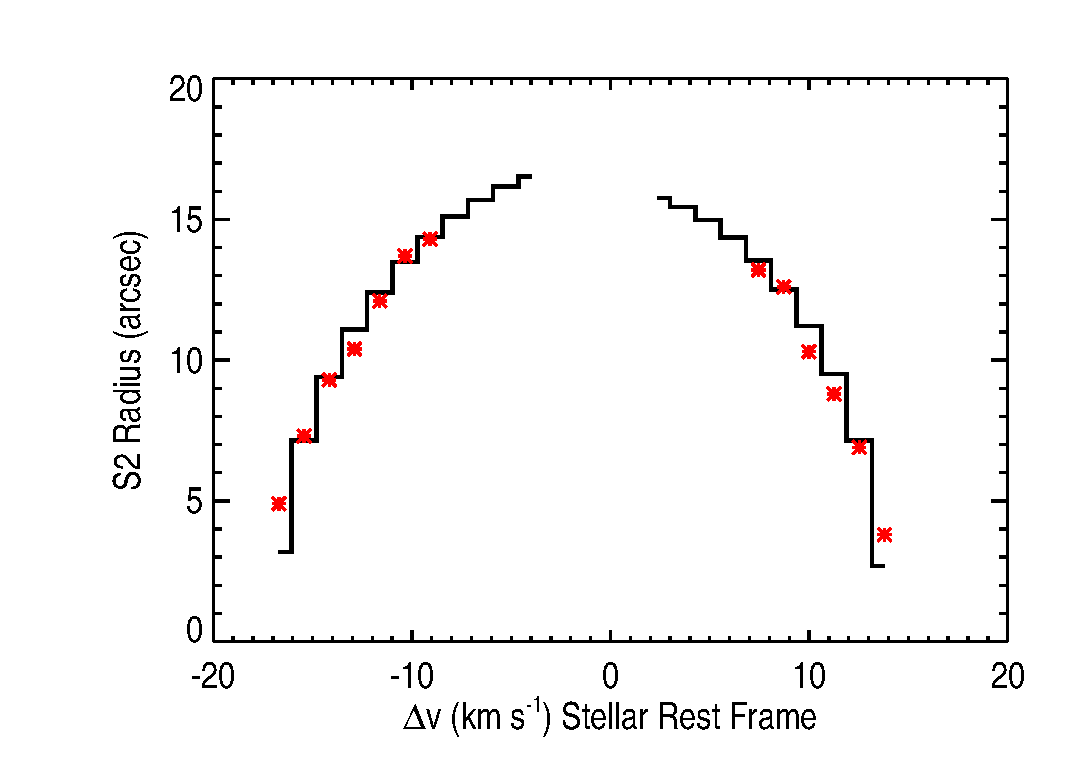
\includegraphics[trim=0pt 0pt 0pt 0pt, clip, scale=0.65]{/home/eamon/thesis/thesis_template/5/f13.eps}
\caption[S2 radius as a function of channel velocity]{The derived S2 radius as a function of velocity (red points) overplotted with two model outflows. The blueshifted model (left) corresponds to an outflow with a maximum radius of 17$\arcsec$ and a velocity of $16.7\>{\rm km\>s}^{-1}$ while the redshifted model (right) corresponds to an outflow with a maximum radius of 16$\arcsec$ and a velocity of $13.8\>{\rm km\>s}^{-1}$. Note: The line profile is $1.9\>{\rm km\>s}^{-1}$ wider in the low resolution image cube ($\Delta v$ = $1.3\>{\rm km\>s}^{-1}$) than in the high resolution image cube.}
\label{fig:5.10}
\end{figure}

%We now use Equation \ref{eq:5.6c} to estimate the maximum projected spatial extent of S2 which occurs at zero velocity.
An estimate of the S2 radius per channel ($r_{\rm{chan}}$) was found by creating annuli of increasing radius around the central emission in each relevant line channel map of the multi-configuration image cube, extracting all flux within each annulus and then plotting these fluxes against distance from the star for each channel map as demonstrated in Figure \ref{fig:5.9}. The maximum of these resultant curves was then deemed to be the maximum radius of S2 per channel map. Figure \ref{fig:5.10} shows these data over-plotted with two model outflows which were created using Equation \ref{eq:5.6c}. The blueshifted data points were best fitted by a model outflow of maximum radius 17$\arcsec$ and outflow velocity $16.7\>{\rm km\>s}^{-1}$, while the redshifted data points were best fitted by a model outflow of maximum radius 16$\arcsec$ and outflow velocity $13.8\>{\rm km\>s}^{-1}$. It is worth mentioning that this estimate for the spatial extent of S2 is only weakly dependent on our adopted radial velocity value for Betelgeuse and adopting a slightly different value would simply alter the outflow velocities.

\section{Intensity distribution of CO}\label{sec:5.7}
We first investigate how one would expect the intensity of CO to vary as a function of distance from the star for a spherically symmetric optically thin outflow. The CO($J=2-1$) emission line is formed over an extended region around Betelgeuse so a constant outflow velocity can be assumed when investigating the intensity distribution of the S1 and S2 outflow. This allows us to use the equation of mass continuity to find the number density of the molecules in the lower level of the transition, $n_{l}$, i.e., $n_{l} \propto r^{-2}$. The Boltzmann formula can then be used to find the number density of CO molecules in the upper level, $n_{u}$, 
\begin{equation}
n_{u}(r)=n_{l}(r)\frac{g_{u}}{g_{l}}e^{-(E_u-E_l)/kT_{\rm{exc}}(r)}
\end{equation}
where $g_{u}$ and $g_{l}$ are the statistical weights of the two rotational levels, and $E_u$ and $E_{l}$ are their respective energies. Here, $T_{\rm{exc}}$ is the excitation temperature and equals to the gas temperature if collisions dominate the redistribution of the populations over the rotational ladder. To find the intensity we first need to know the emissivity, $j_{l}$, of the line photons which is just $n_{u}(r)$ times the probability for spontaneous de-excitation per second, $A_{ul}$, times the energy of the emitted photons, $h\nu$, i.e.,
\begin{align}
j_{l}(r)     & =  n_{u}(r)A_{ul}h\nu \nonumber \\
 &\propto r^{-2}e^{-(E_u-E_l)/kT_{\rm{exc}}(r)}.
\end{align}
If $T_{\rm{exc}}$ is constant then the line intensity, $I_{\rm{CO}}$, can be written as
\begin{align}
I_{\rm{CO}} & = \int j_{l}(r) dr  \nonumber \\
 &\propto r^{-1}.
\end{align}

In the left column of Figure \ref{fig:5.11} we investigate the intensity distribution of CO emission as a function of projected radius, $R$, for both the S1 and S2 flows. From our discussions in Section \ref{sec:5.3} we can assume that all line emission between -15.4 $\rightarrow$ $-10.3\>{\rm km\>s}^{-1}$ and +12.4 $\rightarrow$ $+13.8\>{\rm km\>s}^{-1}$ emanates solely from the S2 flow. Using the low spectral resolution multi-configuration image cube we integrate the surface brightness over these channels and find that the intensity fall-off is close to being proportional to $R{}^{-1}$ (Figure \ref{fig:5.11}: \textit{top left}). To investigate the S1 flow intensity distribution around $\alpha$ Ori we integrate the surface brightness over the channels between -9 $\rightarrow$ $+10.6\>{\rm km\>s}^{-1}$. Although these channels contain emission from both S1 and S2, most of the S2 emission here will have larger projected radii and thus the majority of the inner emission should emanate from the S1 flow.  Between 0.5$\arcsec$ and 4$\arcsec$ from the star the intensity is again found to be close to proportional to $R{}^{-1}$ (Figure \ref{fig:5.11}: \textit{bottom left}). We have just showed that such an intensity distribution is expected for an optically thin homogeneous constant velocity outflow with $\rho \propto 1/\rm{R^{2}}$. Beyond $\sim 6\arcsec$ the intensity fall off is more rapid and is steeper than a $R{}^{-2}$ distribution and may be caused by factors such as a variation in the thermal or velocity profile, or even the absence of emitting material altogether. This region may mark the initiation of the current epoch of mass loss.

\begin{figure}[hbt!]
%\centering
\mbox{
          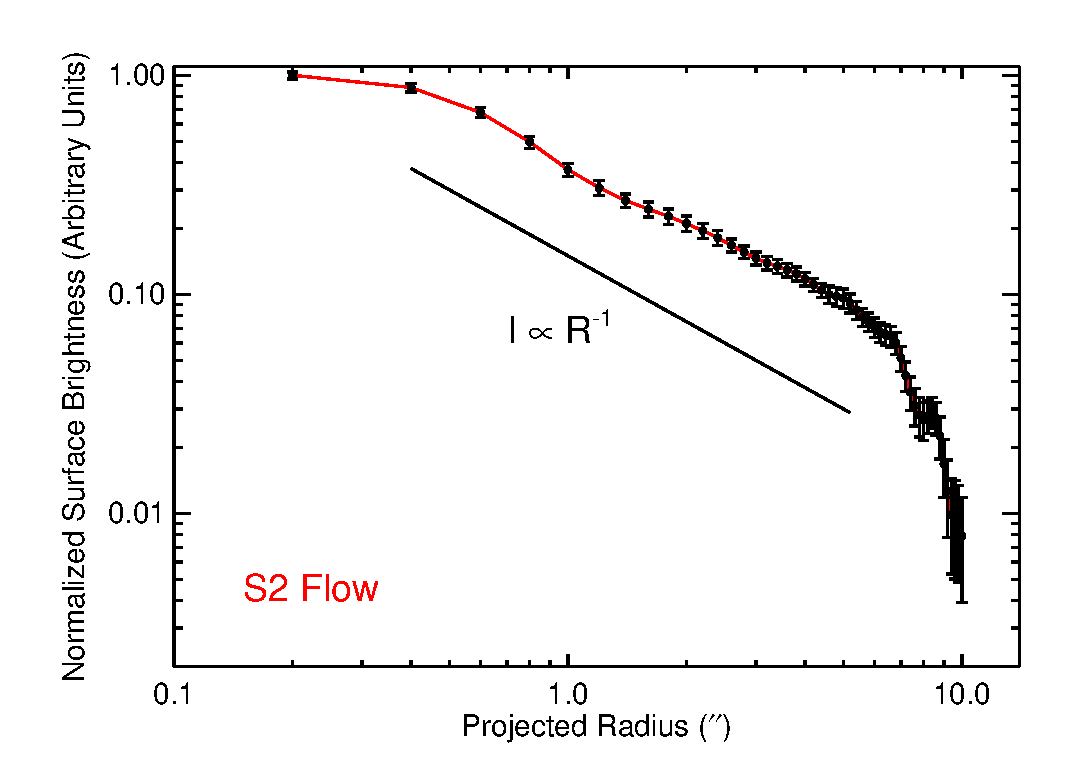
\includegraphics[scale=0.42]{/home/eamon/thesis/thesis_template/5/f14.eps}
          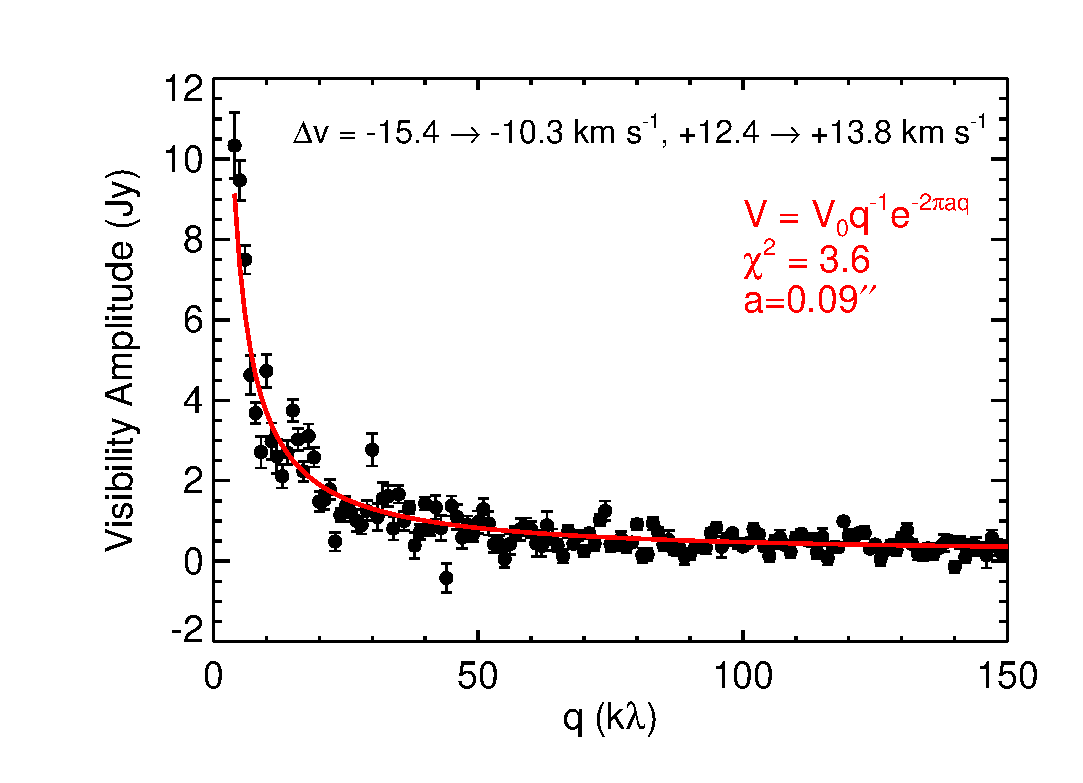
\includegraphics[trim=30pt 0pt 0pt 0pt, clip, scale=0.42]{/home/eamon/thesis/thesis_template/5/f15.eps}
          }
\\
\mbox{
          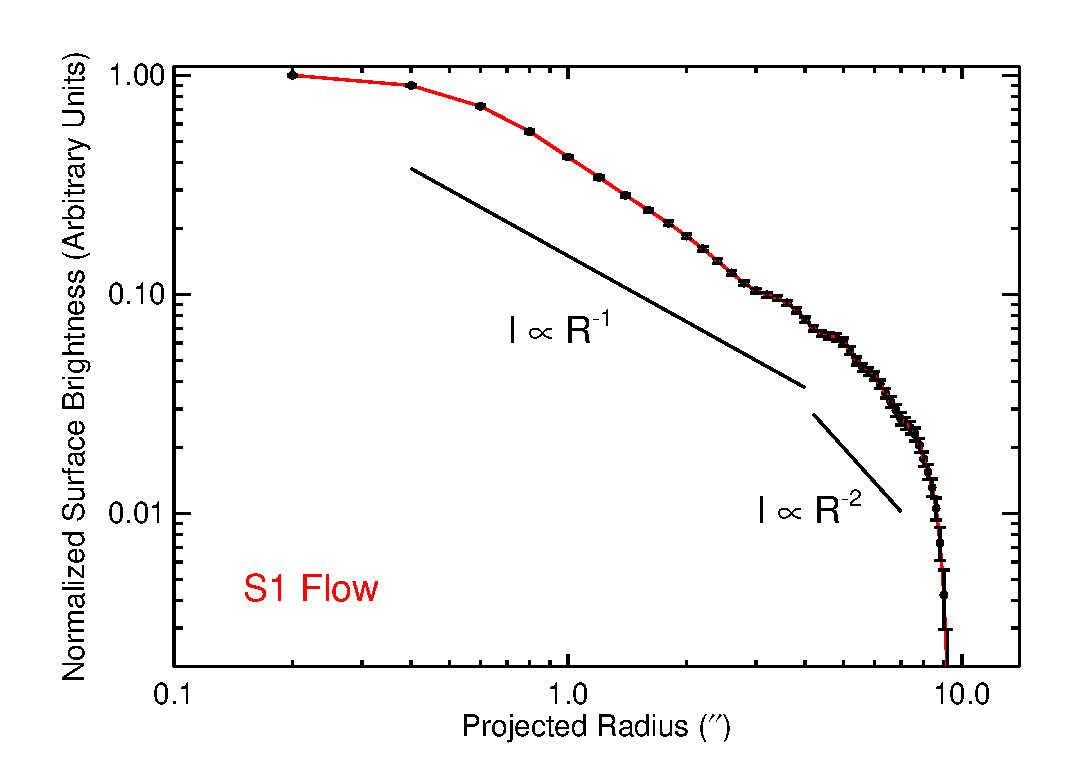
\includegraphics[scale=0.42]{/home/eamon/thesis/thesis_template/5/f16.eps}
          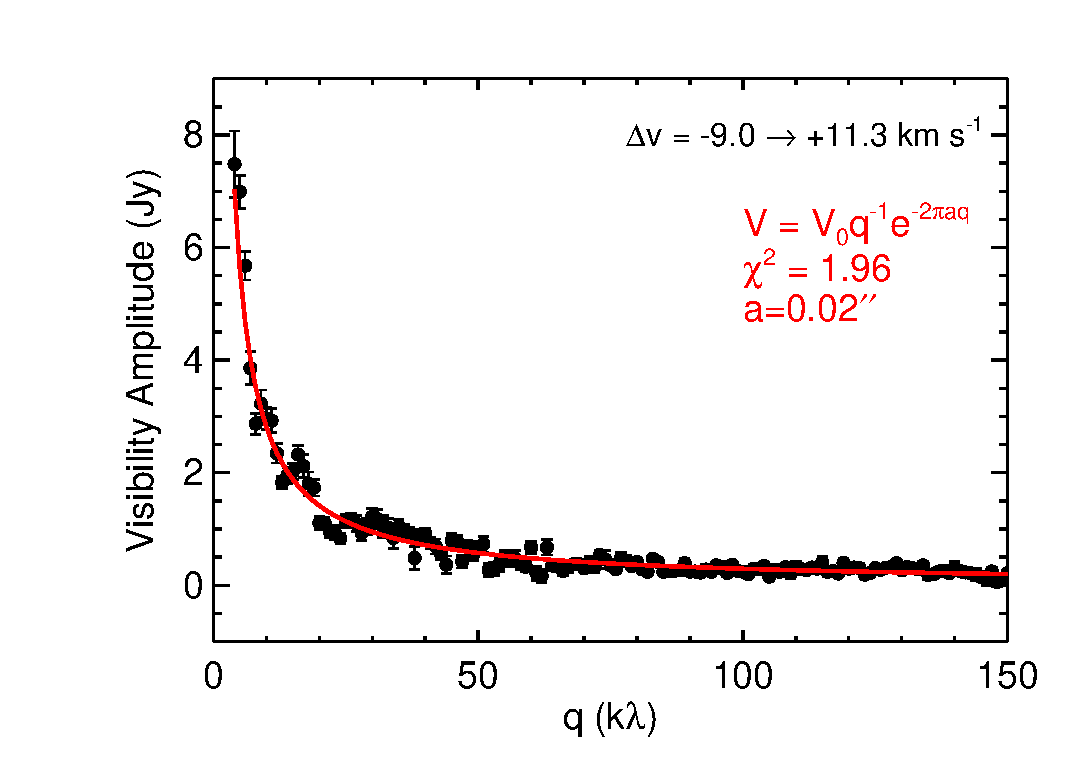
\includegraphics[trim=30pt 0pt 0pt 0pt, clip, scale=0.42]{/home/eamon/thesis/thesis_template/5/f17.eps}

          }
\\
\caption{\textit{Left Column:} Surface Brightness as a function of projected radius on sky, $R$ (red line). The emission has been extracted from the low spectral resolution multi-configuration image cube and is integrated over the channels where S1 is present (bottom) and over the channels where only S2 is present (top). Intensity proportional to $R{}^{-1}$ and $R{}^{-2}$ is also shown for comparison. \textit{Right Column:} The corresponding visibility amplitude as a function of $u-v$ distance ($q$) of both outflows can be modeled well by a $R{}^{-1}$ fall off in intensity. The error bars in all plots represent the standard error of the mean.}
\label{fig:5.11}
\end{figure}

Insight can also be gained into how the intensity varies on different size scales by conducting analysis in the $u-v$ plane and plotting the visibility amplitude of our CO data against $u-v$ distance. The result of this is shown in the right column of Figure \ref{fig:5.11} where the same channels corresponding to the S1 and S2 flows defined in the last paragraph have been used. The data are azimuthally averaged, and have been binned to produce one data point per k$\lambda$. The result for both the S1 and S2 data is a steep drop-off in visibility amplitude over a relatively short $u-v$ distance, signaling that the sources are well resolved, as expected. Both sets of visibility data agree with an intensity proportional to $(a^2 + R^2){}^{-1/2}$, where $a$ is an inner spatial limit. This is because the Hankel transform of this function is $q^{-1}e^{-2\pi aq}$ \citep{bracewell_2000}, where $q$ is the $u-v$ distance, and a vertically scaled version of this function is shown to match the visibility data very well in Figure \ref{fig:5.11}. As analysis in both the sky and $u-v$ plane indicate the intensity of both flows is proportional to $R{}^{-1}$ we conclude that when azimuthally averaged, both outflows are  consistent with an optically thin and quasi-steady flow which is in agreement with \cite{smith_2009} (i.e., S1) and \cite{plez_2002} (i.e., S2). 

\section{Spatial Extent of S1}\label{sec:5.8}
An exact determination of the maximum spatial extent of the S1 flow is more difficult as we do not see the classical shell formation signature for it as we sample across velocities, like we do for S2. Instead its spatial extent varies over the channel maps with evidence of discrete clumps being present in many of these maps. At 20\% of maximum emission in the integrated intensity S1 map (i.e. composed of all channels between -9 $\rightarrow$ $+10.6\>{\rm km\>s}^{-1}$) the S1 flow extends out to a mean distance of $\sim$ 4$\arcsec$ and is even more extended in the S-W direction due to the presence of the second emission feature in the compact configuration data sets. The HPBW of 0.9$\arcsec$ is not sufficient to determine whether the S1 flow is discrete or an extension of the current wind phase seen in ultraviolet spectra, e.g., \cite{1997ApJ...479..970C}, and cm-radio continuum interferometry \citep{1998Natur.392..575L, harper_2001}.

Graham's proceedings
\section{Continuum Flux Densities}\label{sec:5.9}
Betelgeuse is known to show brightness variations at many continuum wavelengths. \cite{goldberg_1984} reports a decrease of half a magnitude in visual brightness over a period of six years. \cite{bookbinder_1987} found stochastic 30\%-40\% variations in flux density at 6\,cm over timescales as short as 10 days to as long as 8 months (i.e. the observational period). A more comprehensive study was carried out by \cite{drake_1992} who observed Betelgeuse with the VLA at centimeter wavelengths from 1986 to 1990 and found stochastic variability of 22\%, 15\%, and 21\% at 6\,cm, 3.6\,cm, and 2\,cm respectively, at a variety of different timescales down to less than one month (a possible source for this variability will be described in Section \ref{sec:5.11}). The mm-continuum emission that we measure arises mainly from electron-ion and electron-atom bremsstrahlung (also the source of the longer wavelength continuum emission) and possibly dust emission, so it is not unreasonable to also expect variability at mm-wavelengths too. 

\begin{table}[!hbt]
\begin{center}
\caption[CARMA Continuum Fluxes at 230 GHz]
{CARMA Continuum Fluxes at 230 GHz between 2007 $\rightarrow$ 2009.}
\begin{tabular}{lcccc}
\hline
\hline
\rule{0pt}{2.5ex}Configuration & Date &Restoring Beam & Flux & Uncertainty \\
 & ($\arcsec \times \arcsec$) & &(mJy) & (mJy) \\
\hline
\rule{0pt}{2.5ex}C & 2007 Jun&0.96 $\times$ 0.76 & 234 & 18\\
D & 2009 Jul&2.33 $\times$ 1.87 & 389 & 72\\
E & 2009 Nov&4.93 $\times$ 3.84 & 278 & 40 \\
Multi-configuration &2007 $\rightarrow$ 2009 &1.05 $\times$ 0.84 & 289 & 21\\
\hline
\rule{0pt}{2.0ex}
\end{tabular}
\label{tab:5.1}
\end{center}
\end{table}


In Table \ref{tab:5.1} we list the derived continuum flux densities for each of the three configuration image cubes and also the multi-configuration image cube. The high spectral resolution ($\Delta v$ = $0.65\>{\rm km\>s}^{-1}$) image cubes were just wide enough to image the CO line but were too narrow to make accurate estimates of the continuum flux density. Therefore, all continuum flux density estimates are derived from the lower spectral resolution ($\Delta v$ = $1.3\>{\rm km\>s}^{-1}$) image cubes from which we were able to take accurate measurements at both sides of the line. We fitted elliptical Gaussians to $\sim$ 20 continuum channels using CASA's \textit{imfit} routine allowing the flux and corresponding uncertainties to be calculated. The source was unresolved in most of these continuum channels. The D configuration data were acquired under adverse weather conditions and these data have the highest noise levels out of the three configurations. Its continuum emission measurement is approximately 50\% greater than the C and E configuration continuum measurements which were also acquired approximately two years after the D configuration data.  We believe the continuum emission value of $289 \pm 21$\,mJy derived from the multi-configuration image cube is a reasonable estimation of the mean mm-continuum flux density over the two year period, 2007 $\rightarrow$ 2009. It is in reasonably good agreement with the 250\,GHz flux density of \cite{altenhoff_1994} who report a mean value of 351$\pm$25\,mJy for 1986 $\rightarrow$ 1989.

\section{Higher CO rotational lines}\label{sec:5.10}
As part of our larger multi-wavelength study of the CO surrounding Betelgeuse we were also able to obtain emission line profiles of higher rotational CO lines. First we observed the star (PI Harper: ID 81-0005-1) with the German Receiver for Astronomy at Terahertz Frequencies \cite[GREAT;][]{guesten_2000} instrument on NASA and DLR's Stratospheric Observatory for Infrared Astronomy \cite[SOFIA;][]{becklin_2009} 2.5\,m airborne observatory. Observations of the  CO($J = 12-11$; 1.38\,THz, $216.9\,\rm \mu m$) line were made during Flight 86 on 2011 November 10 at 13,100\,m ($\sim$ 43,000 ft) when the star had an elevation of 45$^{\circ}$. The HPBW was $\sim 19\arcsec$ and the effective on source exposure time was 12 minutes which was considerably lower than the requested on source time of 70 minutes due to technical difficulties during the flight. We also obtained 4.1 hours on source at 345\,GHz with the Submillimeter Array (SMA) on 2012 January 12 (PI J. Brown: ID 2011B-S051). The SMA is a submillmeter interferometer located  atop Mauna Kea in Hawaii and consists of eight antennas each 6\,m in diameter. Our data was acquired in the compact configuration ($B_{\rm{max}}=70$\,m) which at the observing frequency of $\sim 345$\,GHz gave a synthesized beam of $5\times 4.5$ arcsec$^2$ (similar to the CARMA E configuration at 230\,GHz). We obtained very high spectral resolution ($\Delta v= 0.088$\,km\,s$^{-1}$) of the CO($J = 3-2$; 345.796\,GHz, $866.96\,\rm \mu m$) line which is more than a factor of 7 better than the highest spectral resolution CARMA CO($J = 3-2$) line, and also a weak detection of the SiO($J = 8-7$; 347.3306\,GHz, $863.13\,\rm \mu m$) at a spectral resolution of x\,km\,s$^{-1}$. 
Herschel

% the observations were obtained using a non-standard asymmetric chop sequence with a throw of $60\arcsec$.


\begin{figure}[!ht]
\centering 
\includegraphics[trim=0pt 0pt 0pt 0pt, clip, scale=0.8]{/home/eamon/thesis/thesis_template/5/higher_co_lines.ps}
\caption[]{}
\label{fig:5.12}
\end{figure}

The scaled SOFIA-GREAT emission line profile binned to $1.3\>{\rm km\>s}^{-1}$ is shown in Figure \ref{fig:fig8} along with the CARMA C configuration CO(\textit{J} = 2-1) profile which spatially filters the S2 contribution. This figure shows that the $\textit{J} = 12-11$ profile reflects the slower moving S1 flow with a width of $\sim \pm 7.5\>{\rm km\>s}^{-1}$ approximately centred on the stellar rest frame. This suggests that the $\textit{J} = 12-11$ emitting plasma is not associated with the faster S2 component and is likely associated with the higher excitation S1 plasma. Owing to uncertainties in the pointing accuracy during our GREAT observation we defer a discussion of the fluxes to a later time.

although a search at 86\,GHz for SiO($J= 2-1$) by \cite{lambert_1978} had been unsuccessful
temperatures ratio etc 
\section{CARMA CO observations in Context}\label{sec:5.11}

\section{e-Merlin 6\,cm Results}\label{sec:5.12}
The first detailed study of Betelgeuse at centimeter wavelengths was carried out by \cite{newell_1982}
who observed the star at multiple wavelengths (20, 6, 2, and 1.3\,cm) in a compact VLA configuration. The star was unresolved but a radio spectral index of 1.32 was derived and the radio emission was interpreted as emanating from a spherically symmetric, partially ionized chromosphere with an temperature of  $\sim 10,000$\,K extending from 1 to 4\,$R_{\star}$, in agreement with the Alfv\'en wave models of the time \citep{hartmann_1984}. The star was first spatially resolved at radio wavelengths by \cite{skinner_1997} with both the old VLA in its most extended configuration, and MERLIN (the predecessor to e-MERLIN). The data were taken $\sim 2.5$\,yr apart and it was found that the the 6\,cm radio emitting region was up to three time larger than the optical photosphere. The spatially resolved multi-wavelength study of \cite{lim_1998} revealed a cool, low hydrogen ionization inner atmosphere. To reconcile these observations with spatially resolved UV observations which showed a much warmer (i.e., chromospheric) inner atmosphere, \cite{lim_1998} concluded that there must be at least 3 orders of magnitude more cooler plasma than hot chromospheric plasma, because the radio opacity of the warm gas is much greater than that of the cooler gas. We now discuss the recent findings of \cite{richards_2013} who observed Betelgeuse at 6\,cm with the very long baseline interferometer, e-MERLIN.

\begin{figure}[!ht]
\centering 
\mbox{
          \includegraphics[trim=130pt 280pt 90pt 280pt,clip,width=8.8cm,height=7.8cm]{/home/eamon/thesis/thesis_template/5/emerlin_im.ps}
          \includegraphics[trim=30pt 80pt 0pt 50pt,clip,width=6.0cm,height=9.0cm]{/home/eamon/thesis/thesis_template/5/emerlin_vis.ps}
          }
\caption[First e-MERLIN results for Betelgeuse.]{First e-MERLIN results for Betelgeuse. \textit{Left:} 5.2\,cm e-MERLIN image of Betelgeuse taken in July 2012 showing two unresolved emission features separated by $90\pm10$\,mas. The image was restored with a $80\times 60$\,mas$^2$ beam marked in green in the lower left corner and using uniform weighting. Contour levels are at $(-3, 3, 6, 12, 24, 48)\times \sigma _{\rm{rms}}$ where $\sigma _{\rm{rms}} = 9\mu$\,Jy. The photospheric radius is the small black circle which the large yellow circle defines the 6\,cm radio disk of \cite{lim_1998}. \textit{Right:} The calibrated visibility amplitudes (in mJy) versus $u-v$ distance measured in mega-wavelengths with the possible signature of two unresolved components with a brightness ratio differing from unity. }
\label{fig:5.13}
\end{figure}

e-MERLIN \citep{muxlow_2003} consists of seven radio antennas spread out across the United Kingdom that are connected via a fiber optic network to a central correlator at Jodrell Bank Observatory. It will eventually be able to observe in three frequency bands at $1.3-1.8$\,GHz, $4-8$\,GHz, $22-24$\,GHz, and its maximum baseline of 220\,km will provide resolution up to 10\,mas at the $\mu$Jy sensitivity level. Betelgeuse was observed at 5.76\,GHz (5.2\,cm) in 2012 July with e-MERLIN as part of Cycle-0 observations, with a total bandwidth of 0.512\,GHz. The final high resolution image which is shown in Figure \ref{fig:5.13} had a $\sigma _{\rm{rms}}=9\mu$\,Jy and was produced using uniform weighting using a restoring beam of ($80\times 60$) mas$^2$. The first thing to notice about the radio map is the presence of three clumps of radio emission in the south-west quadrant approximately 250\,mas (11.5\,$R_{\star}$) from the star, with detections ranging from 4 to $12\sigma _{\rm{rms}}$. These clumps of radio emitting plasma are probably the remnants of past localized episodic mass loss events from the star, which as they escaped the gravitational potential of the star, expanded, cooled allowing hydrogen to recombine and thus in the process becoming fainter radio continuum emitters than they initially were. Assuming a mean constant flow velocity of 5\,km\,s$^{-1}$ \citep[see Figure 10 in][]{harper_2001}, then this plasma was ejected from the star $\sim 45$\, yr prior to these observations but could be almost double this value if the slow wind acceleration profile given in \cite{harper_2001} is assumed.

The second and more remarkable feature of the image is that the star at 6\,cm appears as two unresolved peaks separated by $\sim 90$\,mas. To make sure this unexpected result was not an artifact of the imaging process we plotted the visibility amplitude as a function of baseline (i.e., $\sqrt{u^2 + v^2}$) as shown also in Figure \ref{fig:5.13}. If we had resolved a standard uniform disk, which should be a good first order approximation for any \textit{standard} star, then we would expect the visibility amplitude to drop to zero at some stage, which clearly does not happen. On the other hand, the visibility amplitude for a double source would depict two peaks with the minimum visibility amplitude being a function of the component brightness ratio. For equal brightness (i.e., the ratio is 1) the first visibility amplitude minimum drops to zero but does not for sources of different brightness \citep{saha_2011}. Therefore, the visibility amplitudes of our our calibrated data appear to be in agreement with what is seen in the final image, i.e., two sources of different brightness producing a sinusoidal visibility pattern which does not drop to zero. 

\begin{figure}[!ht]
\centering 
          \includegraphics[trim=0pt 50pt 40pt 50pt,clip,width=10.0cm,height=12.0cm,angle=90]{/home/eamon/thesis/thesis_template/5/merlin_parallax.ps}
\caption[Predicted position of Betelgeuse on 2012 July using the astrometric solutions of \cite{harper_2001}.]{The red filled circle marks the predicted position of the optical photosphere of Betelgeuse on 2012 July using the astrometric solutions of \cite{harper_2001}. The black contours represent the high spatial resolution 6\,cm image of the star from \cite{richards_2013} and are at the $4\sigma _{\rm{rms}}$ level. This solution puts the optical photospheric position almost at the position of the weaker unresolved peak.}
\label{fig:5.14}
\end{figure}

The brighter feature was found to have a brightness temperature of $T_{\rm{b}}=5,400\pm 600$\,K while the weaker feature had $T_{\rm{b}}=3,800\pm 500$\,K. To find the position of the optical photosphere, \cite{richards_2013} took the peak flux position from a low resolution radio map which was optimized for sensitivity to extended structure. In this scenario the two features, referred to as \textit{hotspots} by \cite{richards_2013} are located 1.0 ($T_{\rm{b}}=5,400$\,K) and 1.5\,$R_{\star}$ ($T_{\rm{b}}=3,800$\,K) from the optical photosphere. A more rigorous approach to finding the position of the optical photosphere is to use the astrometric solutions derived in a study to find the distance to Betelgeuse \citep[solution 5 in][]{harper_2008} and propagate these forward to find its expected position in 2012 July. Doing this we get RA\,$=05:55:10.3250$ and dec\,$=+07:24:25.536$ which includes the correction for parallax. We plot this expected position on top of the e-MERLIN map in Figure \ref{fig:5.14}. Interestingly, this puts the expected optical photospheric position almost directly on top of the weaker emission feature. The effective temperature of Betelgeuse is 3,650\,K \citep{levesque_2005} which is slightly below the brightness temperature derived for this feature but well within its errors (i.e., $T_{\rm{b}}=3,800\pm 500$\,K). If this weaker source is indeed the optical photosphere, then the brighter source with $T_{\rm{b}}=5,400\pm 600$\,K is located at least $3.5\,R_{\star}$ from the surface of the optical photosphere. Its value is significantly higher than that predicted in the spherically symmetric semi-empirical model of \cite{harper_2001} who predict a value of 2,300\,K at a projected radius of 95\,mas (i.e., $3.5\,R_{\star}$ from the photosphere).

\begin{figure}[!ht]
\centering 
          \includegraphics[trim=0pt 50pt 0pt 0pt,clip,width=12.0cm,height=15.0cm,angle=90]{/home/eamon/thesis/thesis_template/5/3_plots_new.ps}
\caption[]{\textit{Left column:} Two-dimensional specific intensity contour maps at 5.2\,cm (5.75\,GHz) created using the one-dimensional inner atmospheric model of Betelgeuse by \cite{harper_2001} described in the text. The maps have been convolved with a beam having dimensions ($80\times 60$) mas$^2$ (top) and ($180\times 180$) mas$^2$ (bottom). \textit{Right column:} The observed high (top) and low (bottom) resolution e-MERLIN images. The high resolution image is a poorly described by the model of \cite{harper_2001} highlighting the inadequacies of one-dimensional spherically symmetric models in describing the inner atmosphere of Betelgeuse.}
\label{fig:5.15}
\end{figure}

The semi-empirical model of \cite{harper_2001} is the current \textit{state of the art} inner (i.e., $1 \rightarrow 10\,R_{\star}$) atmospheric model for Betelgeuse. It consists of a detailed mean density and temperature one-dimensional model and is based on the spatially resolved VLA data of \cite{lim_1998}. In this model the temperature distribution peaks at 1.45\,$R_{\star}$ where it reaches $\sim 3800$\,K and decreases to $\sim 3800$\,K at 10\,$R_{\star}$. The dominant source of electrons is from photoionized metals while hydrogen has a low level of ionization. 
We use this model to create a two-dimensional spherically symmetric specific intensity map to examine how it compares with the new e-MERLIN high resolution data at 5.2\,cm (5.75\,GHz). As shown in Figure \ref{fig:5.15}, we convolved this map with a restoring beam, first with dimensions ($180\times 180$) mas$^2$ to match the low resolution e-MERLIN image and then with dimensions ($80\times 60$) mas$^2$ to match the high resolution e-MERLIN image. As can be seen from Figure  \ref{fig:5.15}, the atmospheric model of \cite{harper_2001} does a good job in reproducing the low resolution e-MERLIN image but, as would be expected from a spherically symmetric 1-D model, fails to reproduce the more complex structure which is seen in the higher resolution e-MERLIN image. The advent of the new e-MERLIN interferometer with its superior spatial resolution to that of the VLA has revealed that 1-D spherically symmetric atmospheric models are probably hopelessly inadequate in describing the inner atmospheric conditions of Betelgeuse. Time dependent models which radically diverge from spherical symmetry will ultimately be needed to accurately describe the inner atmospheric conditions of Betelgeuse.

\section{Multi-wavelength VLA-Pie Town Results}\label{sec:5.13}
At the end of Chapter \ref{chap:3} we describe the VLA-Pie Town observations of Betelgeuse from the early 2000's along with the motivation for analyzing it. In summary, we wanted to see if there was some signature of the e-MERLIN asymmetries in the data set, because the Pie-Town link when connected to the VLA provided resolution comparable to or exceeding that of the e-MERLIN data set at the shortest wavelengths.

\subsection{Confirmation of a Low Temperature Wind}
\subsection{Flux Density Variability}
\subsection{High Resolution Maps}

Should be roughly 50 mas from optical photosphere. No assymetries present. Therefore ballistic ejection or looking into deeper cooler layers?? too many uncertainties with the time difference between them too long